% !TeX program = pdflatex
\documentclass[border=6pt]{standalone}
\usepackage{tikz}
\usetikzlibrary{arrows.meta, positioning, calc}

\definecolor{MediumRed}{rgb}{0.925, 0.345, 0.345}
\definecolor{MediumGreen}{rgb}{0.37, 0.7, 0.66}
\definecolor{MediumBlue}{rgb}{0.015, 0.315, 0.45}
\definecolor{DarkBlue}{rgb}{0.05, 0.15, 0.35}

\begin{document}
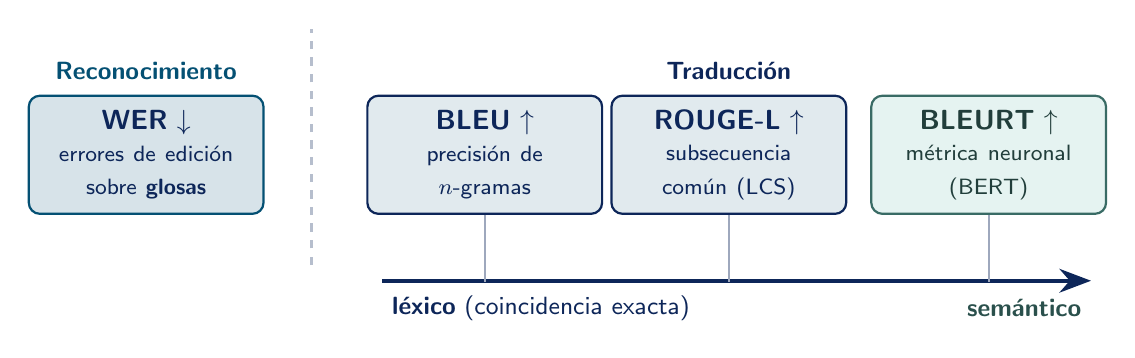
\begin{tikzpicture}[
    font=\sffamily,
    badge/.style={draw=DarkBlue, thick, rounded corners=4pt, fill=MediumBlue!12,
        text=DarkBlue, align=center, text width=2.7cm, minimum height=1.5cm, inner sep=4pt},
]

% ---- Reconocimiento (glosas) ----
\node[badge, draw=MediumBlue, fill=MediumBlue!16] (wer) at (0,0)
    {\textbf{WER} $\downarrow$\\[2pt]\footnotesize errores de edición\\\footnotesize sobre \textbf{glosas}};
\node[font=\sffamily\small\bfseries, text=MediumBlue, above=2pt of wer] {Reconocimiento};

% separador
\draw[DarkBlue!30, thick, dashed] (2.1,-1.4) -- (2.1,1.6);

% ---- Traducción: eje léxico -> semántico ----
\draw[-{Stealth[length=4mm]}, line width=1.6pt, DarkBlue] (3.0,-1.6) -- (12.0,-1.6);
\node[font=\sffamily\small, text=DarkBlue, anchor=west]  at (3.0,-1.95) {\textbf{léxico} (coincidencia exacta)};
\node[font=\sffamily\small, text=MediumGreen!45!black, anchor=east] at (12.0,-1.95) {\textbf{semántico}};

\node[badge] (bleu) at (4.3,0)
    {\textbf{BLEU} $\uparrow$\\[2pt]\footnotesize precisión de\\\footnotesize $n$-gramas};
\node[badge] (rouge) at (7.4,0)
    {\textbf{ROUGE-L} $\uparrow$\\[2pt]\footnotesize subsecuencia\\\footnotesize común (LCS)};
\node[badge, draw=MediumGreen!60!black, fill=MediumGreen!16, text=MediumGreen!35!black] (bleurt) at (10.7,0)
    {\textbf{BLEURT} $\uparrow$\\[2pt]\footnotesize métrica neuronal\\\footnotesize (BERT)};
\node[font=\sffamily\small\bfseries, text=DarkBlue, above=2pt of rouge] {Traducción};

\foreach \m in {bleu,rouge,bleurt} \draw[DarkBlue!40, thick] (\m.south) -- ($(\m.south)-(0,0.85)$);

\end{tikzpicture}
\end{document}
